\chapter{Разработка приложения} \label{chapt3}

Приложение логически делится на две большие части - серверную и клиентскую. В этой главе будут рассмотрены детали работы каждой из этих частей, а также сценарии их взаимодействия.

\section{Модули серверной части} \label{sect3_1}

Под серверной частью понимается совокупность скриптов на языке Python, отвечающая за следующие задачи:

\begin{itemize}
  \item Работа веб-сервера
  \item Управление запуском и остановкой программ RTKRCV, STR2STR и CONVBIN пакета RTKLIB
  \item Чтение и создание конфигурационных файлов для RTKRCV
  \item Управление сохраненными на устройстве логами ГНСС данных
\end{itemize}


\begin{itemize}
  \item Не вмешиваться в сложную внутреннюю структуру приложения, рискуя что-то нарушить
  \item Сохранить совместимость с новыми версиями RTKLIB, даже при серьезных изменения кодовой базы
  \item Писать веб-приложение на более подходящем для этого языке
  \item Не добавлять никакие дополнительные механизмы IPC в RTKLIB
\end{itemize}


\subsection{Низкоуровневая работа с RTKLIB. Класс RtkController} \label{subsect3_1_1}

В качестве основного средства извлечения контроля над программами пакета RTKLIB была выбрана библиотека Pexpect. Pexpect предоставляет возможность автоматизировать работу с интерактивными терминальными приложениями с помощью простой логики ожидания. Например, при запуске RTKRCV пользователь попадает в интерактивную консоль. Также, как и многие стандартные командные оболочки, к примеру \textbf{BASH}, перед ожиданием новой команды пользователя, RTKRCV выводит специальную последовательность символов - \textbf{rtkrcv>}. Pexpect предлагает следующую модель взаимодействия - отправить команду, а затем ждать контрольную строчку, показывающую что предыдущая команда обработана, а подконтрольное приложение готово принимать следующую. В приложении есть три класса, инкапсулирующие взаимодействие с программами RTKLIB: \textbf{RtkController} работает с RTKRCV, \textbf{Str2StrController} c STR2STR, \textbf{ConvbinController} с CONVBIN. Все они обладают свойством child, которому присваивается объект класса \textbf{Pexpect.spawn}. Например, функция, запускающая RTKRCV выглядит вот так:

\lstinputlisting[
  label={listings:RtkController_launch},
  caption={Метод launch класса RtkContoller},
  style={java}
]
{src/RtkController_launch.py}

Главная строка в этой функции - четырнадцатая. Именно здесь, в конструкторе класса \textbf{pexpect.spawn} происходит вызов программы RTKRCV с помощью команды из переменной \textbf{spawn\textunderscore command}. С помощью ключа «-o» указывается конфигурационный файл для загрузки. Следующий важный этап - проверка запуска на ошибку. Это происходит в функции \textbf{self.expectAnswer("spawn")}. Рассмотрим эту функцию подробнее:

\begin{ListingEnv}[H]
  \caption{Метод expectAnswer класса RtkController}
  \label{list:hwbeauty}
  \begin{lstlisting}[language=Python]
    def expectAnswer(self, last_command = ""):
        a = self.child.expect(["rtkrcv>", pexpect.EOF, "error"])
        # check rtklib output for any errors
        if a == 1:
            print("Encountered exception: " + str(self.child))
            return -1

        if a == 2:
            return -2

        return 1
  \end{lstlisting}
\end{ListingEnv}

Кроме возврата кода ошибки(или успеха) операции, вызывает метод expect класса \textbf{pexpect.spawn}. В качестве единственного параметра указан список строк. Метод \textbf{expect} читает стандартный вывод запущенной программы и ждет одну из этих строк. Под опцией \textbf{pexpect.EOF} понимается окончание работы программы. Таким образом, мы получаем представление о том, что же произошло с программой, запущенной с помощью \textbf{pexpect.spawn}.

Кроме того, чтобы запускать программу RTKRCV, мы должны также с ней взаимодействовать. Как только мы увидели, что вывод программы дошел до строки \textbf{rtkrcv>}, программа готова для дальнейшего взаимодействия. RTKRCV предлагает следующие команды консоли:

\begin{itemize}
  \item start. Запустить вычисления координат
  \item stop. Остановить вычисления
  \item load. Загрузить конфигурационный файл
  \item status. Получить статус вычислений в виде текста
  \item obs. Получить информацию о принимаемых сигналах спутников
  \item shutdown. Завершить работу приложения
\end{itemize}

Рассмотрим примеры работы с командами интерактивной консоли. Команды start, stop, load и shutdown работают по одной схеме: отправить команду, дождаться следующего вывода ключевой строки. К примеру, функция, запускающая вычисления:

\begin{ListingEnv}[H]
  \caption{Метод start класса RtkController}
  \label{list:hwbeauty}
  \begin{lstlisting}[language=Python]
    def start(self):
      if not self.started:
        self.semaphore.acquire()
        self.child.send("start\r\n")

        if self.expectAnswer("start") < 0:
          self.semaphore.release()
          return -1

        self.semaphore.release()
        self.started = True
        return 1

      # already started
      return 2
  \end{lstlisting}
\end{ListingEnv}

Взаимодействие происходит по той же схеме - отправление команды, ожидание ответа. Если ответ не содержит слово \textbf{error} (RTKLIB всегда сообщеает об ошибке в стандартный вывод), а приложение неожиданно не закончило свою работу, команда выполнена успешно.

Кроме таких команд, для которых требуется лишь подтверждение отсутствия ошибки, есть команды status и obs. Они возвращают полезную информацию, которую следует прочитать и распарсить. Информация, полученная с помощью команды status понадобится для отображения текущий координаты и качества решения. Obs возвращает таблицу, которая в том числе содержит signal to noise ratio(SNR), то есть уровни видимости спутников. Эта информация будет использоваться для графика на клиентской части приложения. Общий принцип работы такой же: отправить команду, дождаться ответа. Только теперь, нужно пройти по всему выводу программы после отправки команды и выделить из него полезную информацию.

\begin{ListingEnv}[H]
  \caption{Метод getStatus класса RtkController}
  \label{list:hwbeauty}
  \begin{lstlisting}[language=Python]
    def getStatus(self):
      self.semaphore.acquire()
      self.child.send("status\r\n")

      if self.expectAnswer("get status") < 0:
          self.semaphore.release()
          return -1

      status = self.child.before.split("\r\n")
      if status != {}:
          for line in status:
              spl = line.split(":")

              if len(spl) > 1:
                  param = spl[0].strip()
                  value = spl[1].strip()

                  self.status[param] = value

      ...
  \end{lstlisting}
\end{ListingEnv}

Известно, что вывод команды status представляет собой набор строк, в которых параметр и его значение разделены двоеточиями. После получения подтверждения об отсутствии ошибки в выполнении, функция обращается к свойству \textbf{before}, представляющую весь вывод в виде одной строки. С помощью команды \textbf{split("\textbackslash r\textbackslash n")} можно разделить весь вывод на список отдельных строк, а затем обратиться к каждой из них с помощью цикла for. Если строка делится на две по символу «\textbf{:}», значит она содержит пару параметр-значение и подходит для добавление во внутреннюю переменную класса RtkController - status.

Работа с остальными программами RTKLIB - STR2STR и CONVBIN происходит ровно таким же образом, за тем исключением, что они не интерактивны и автоматизация ограничивается запуском с правильными ключами и параметрами, а также чтением результатов работы из стандартного вывода.

\subsection{Работа с конфигурационными файлами. Класс ConfigManager} \label{subsect3_1_2}

Как уже упоминалось, RTKRCV использует конфигурационные файлы для хранения и изменения многочисленных настроек. Приложение должно уметь читать эти файлы, для того чтобы правильно отображать эти настройки в клиентской части, а также перезаписывать измененые в браузере значения. Для этого создан класс ConfigManager. Он служит для того, чтобы:

\begin{itemize}
  \item Возвращать список доступных конфигурационных файлов
  \item Читать файлы и возвращать словарь настроек
  \item Создавать файл из словаря настроек
  \item Сбросить файл до значения по умолчанию
  \item Удалить файл
\end{itemize}

Для работы этого класса используется вспомогательный класс \textbf{Config}, который принимает путь к конфигурационному файлу как единственный параметр конструктора и прочитав файл, создает словарь значений. Рассмотрим пример конфигурационного файла RTKRCV:

\begin{ListingEnv}[H]
  \caption{Отрывок конфигурационного файла RTKRCV}
  \label{list:hwbeauty}
  \begin{lstlisting}[language=Python]
    inpstr1-type       =serial     # (0:off,1:serial,2:file,3:tcpsvr,4:tcpcli,7:ntripcli,8:ftp,9:http) ## Input source for onboard receiver
    inpstr2-type       =tcpcli     # (0:off,1:serial,2:file,3:tcpsvr,4:tcpcli,7:ntripcli,8:ftp,9:http) ## Input source for base corrections
    inpstr3-type       =off        # (0:off,1:serial,2:file,3:tcpsvr,4:tcpcli,7:ntripcli,8:ftp,9:http)
    inpstr1-path       =ttyMFD1:230400:8:n:1:off
  \end{lstlisting}
\end{ListingEnv}

У некоторых строк есть комментарии. Эти комментарии, отделенные одним символом \textbf{\#}, показывают возможные варианты значений параметра. Комментарии отделенные \textbf{\#\#}, используются для подписей параметров в форме на веб-странице. При чтении файла, каждая строка читается и собирается в словарь с четырьмя полями.

\begin{ListingEnv}[H]
  \caption{Представление параметра конфигурационного файла в памяти}
  \label{list:hwbeauty}
  \begin{lstlisting}[language=Python]
  item0 = {
    "parameter": "p",
    "value": "v",
    "comment": "c",
    "description": "d"
  }
  \end{lstlisting}
\end{ListingEnv}

Этот класс используется более общим классом RTKLIB, речь о котором пойдет в следующей части.

\subsection{Высокоуровневая работа с RTKLIB. Класс RTKLIB} \label{subsect3_1_4}

Класс RTKLIB берет на себя почти все функции, связанные с управлением RTKLIB. Через методы и свойства этого класса сервер

Рассмотрим основные функции класса RTKLIB:

\begin{itemize}
  \item Переключение между режимами ровера и базы
  \item Запуск и остановка ровера и базы
  \item Чтение и запись настроек роверка и базы
  \item Конвертация логов данных в другой формат
  \item Сохранение и загрузка режима работы
  \item Трансляция координат и уровней спутников на фронтэнд
\end{itemize}

Основной задачей этого класса является объединение множества разрозненной функциональности в одно место, а также инкапсуляция всех нюансов работы с отдельными частями RTKLIB. Например этот класс берет на себя обработку ошибок в работе классов более низкого уровня.

Одни из самых главных понятий, определенных в классе RTKLIB - состояния ровера и базы. Дело в том, что RTKLIB сам по себе не предполагает таких ролей. Есть RTKRCV, занимающийся расчетом координат с помощью совмещения показаний двух приемников. Также есть STR2STR, который позволяет перенаправлять потоки данных ГНСС приемников. Однако, STR2STR - единственная программа пакета, которая способна выдавать данные в легковесном формате RTCM3. Поэтому в классе RTKLIB запуск режима ровера равносилен запуску RTKRCV с помощью класса RtkController, а запуск режима базы - запуску STR2STR с помощью Str2StrController.

Функции записи настроек - writeConfigRover или writeConfigBase передают управление различным классам более низкого уровня - ConfigManager и Str2StrController. Причина этого кроется в том, что STR2STR не нуждается в конфигурационных файлах. Все настройки передаются через параметры запуска приложения. Таким образом, в случае с ровером нужна перезапись файла на диске, а в случае с базой - достаточно изменить свойства класса Str2StrController.

Кроме передачи управления другим классам у RTKLIB есть своя уникальная функциональность. Например, с помощью функций \textbf{saveState} и \textbf{loadState}, класс записывает и загружает все настройки. Если настройки RTKRCV сохраняются в файлы, то остальные настройки, такие как режим базы или ровера, а также настройки базы, надо хранить отдельно. При выполнении любой операции, затрагивающей изменения настроек вызывается \textbf{saveState}. Внутри функции информация собирается в словарь, который переводится в JSON формат с помощью стандартного модуля \textbf{json}. При загрузке, которая проходит при запуске приложения этот файл считывается, JSON декодируется обратно в Python словарь и запускаются соответствующие методы класса RTKLIB, чтобы продолжить работу с том же состоянии. Это очень полезно, если приложение запускается при загрузке операционной системы. Таким образом, можно продолжать работу в том же режиме после включения устройства без необходимости залезать в настройки.

Еще одна важная функция, которую на себя берет класс RTKLIB - трансляция координат и уровней спутников в браузер посредством веб-сокетов. При старте в режиме ровера, создаются и запускаются два новых потока: \textbf{satellite\_ thread} и \textbf{coordinate\_ thread}. Эти потоки выполняют методы класса RTKLIB \textbf{broadcastCoordinates} и \textbf{broadcastSatellites}. Рассмотрим одну из них:

\begin{ListingEnv}[H]
  \caption{Метод broadcastSatellites класса RTKLIB}
  \label{list:hwbeauty}
  \begin{lstlisting}[language=Python]
    def broadcastSatellites(self):
      count = 0
      while self.server_not_interrupted:
        self.rtkc.getObs()
        if count % 10 == 0:
          print("Sending sat rover levels:\n" + str(self.rtkc.obs_rover))
          print("Sending sat base levels:\n" + str(self.rtkc.obs_base))

        self.socketio.emit("satellite broadcast rover", self.rtkc.obs_rover, namespace = "/test")
        self.socketio.emit("satellite broadcast base", self.rtkc.obs_base, namespace = "/test")
        count += 1
        time.sleep(1)
  \end{lstlisting}
\end{ListingEnv}

Эта функция заключается в бесконечном цикле, постоянно считывающем статус из RTKRCV и отправлюящем его в браузер с помощью объекта \textbf{socketio}. В случае остановки в режиме ровера, свойство \textbf{server\_ not\_ interrupted} становится \textbf{False} и поток заканчивает свое выполнение.

\subsection{Запуск главной программы и сервера. Модуль server.py} \label{subsect3_1_5}

Главным файлом в проекте является \textbf{server.py}. Основными функциями модуля являются:

\begin{itemize}
  \item Создание и запуск сервера
  \item Инициализация объекта класса RTKLIB для работы с RTK функциями
  \item Создание обработчиков HTTP запросов
  \item Создание обработчиков WebSocket событий
\end{itemize}

Инициализация объекта сервера:

\begin{ListingEnv}[H]
  \caption{Инициализация сервера}
  \label{list:hwbeauty}
  \begin{lstlisting}[language=Python]
    from flask import Flask, render_template, session, request, send_file
    from flask.ext.socketio import SocketIO, emit, disconnect
    from subprocess import check_output

    app = Flask(__name__)
    app.template_folder = "."
    app.debug = False
    ...

    socketio = SocketIO(app)
  \end{lstlisting}
\end{ListingEnv}


Фрэймворк Flask имеет модульную архитектуру, поэтому WebSocket функциональность реализована в расширении Flask-socketio. Для того чтобы подключить данное расширение, следует передать объект класса Flask в конструктор класса SocketIO. После этого переменная \textbf{app} имеет возможность обрабатывать события, связанные с веб-сокетами.

Так как предложение имеет лишь одну страницу, а вся навигация происходит строго в браузере, то на сервере зарегистрированы лишь два обработчка HTTP запросов - для самой страницы:

\begin{ListingEnv}[H]
  \caption{Обработчик HTTP запроса в Flask приложении}
  \label{list:hwbeauty}
  \begin{lstlisting}[language=Python]
    @app.route("/")
    def index():
      rtk.logm.updateAvailableLogs()
      return render_template("index.html", logs = rtk.logm.available_logs, system_status = reach_tools.getSystemStatus())
  \end{lstlisting}
\end{ListingEnv}

И для скачивания логов:

\begin{ListingEnv}[H]
  \caption{Обработчик HTTP запроса в Flask приложении}
  \label{list:hwbeauty}
  \begin{lstlisting}[language=Python]
    @app.route("/logs/download/<path:log_name>")
    def downloadLog(log_name):
      full_log_path = rtk.logm.log_path + "/" + log_name
      return send_file(full_log_path, as_attachment = True)
  \end{lstlisting}
\end{ListingEnv}

Практически весь остальной код данного модуля - регистрация обработчиков событий, связанных с веб-сокетами. Синтаксис у них такой же. Например, событие запуск режима ровера обрабатывается вот так:

\begin{ListingEnv}[H]
  \caption{Обработчик HTTP запроса в Flask приложении}
  \label{list:hwbeauty}
  \begin{lstlisting}[language=Python]
    @socketio.on("launch rover", namespace="/test")
    def launchRover():
        rtk.launchRover()
  \end{lstlisting}
\end{ListingEnv}

Следует обратить внимание на особенность синтаксиса в этих примерах. Декораторы используются для привязки нижеописанных функций к событиям, переданным в качестве параметров декоратору.

Главный цикл крайне прост. Он всего лишь запускает сервер и обрабатывает исключение KeyboardInterrupt(нажатие CTRL+C), корректно завершая все потоки. Это полезное дополнение при разработке.

\begin{ListingEnv}[H]
  \caption{Главный цикл}
  \label{list:hwbeauty}
  \begin{lstlisting}[language=Python]
    if __name__ == "__main__":
      try:
        socketio.run(app, host = "0.0.0.0", port = 80)
      except KeyboardInterrupt:
        rtk.server_not_interrupted = False
        rtk.led.blinker_not_interrupted = False
        rtk.waiting_for_single = False

        if rtk.coordinate_thread is not None:
            rtk.coordinate_thread.join()

        if rtk.satellite_thread is not None:
            rtk.satellite_thread.join()

        if rtk.led.blinker_thread is not None:
            rtk.led.blinker_thread.join()

  \end{lstlisting}
\end{ListingEnv}

\section{Веб-страница и модули клиентской части} \label{sect3_2}

Под клиентской частью понимается веб-страница и совокупность скриптов на языке Javascript, отвечающие за следующие задачи:

\begin{itemize}
  \item Отображение статуса RTKLIB
  \item Отображение форм настройки RTKLIB
  \item Отображение списка логов данных
\end{itemize}

\subsection{Основа клиентской части - HTML страница} \label{subsect3_2_1}

Весь интерфейс приложения строится вокруг одной HTML страницы. Все элементы на странице выбраны из стандартных элементов UI фрэймворка jQuery Mobile. Общая структура документа - несколько \textbf{div} элементов со свойством \textbf{data-role} выставленным на значение \textbf{"page"}. Это дает возможность перемещаться между различными экранами без необходимости перезагрузки страницы, или обращения к серверу, как к таковому.

\begin{ListingEnv}[H]
  \caption{Создание элемента-страницы в jQuery Mobile}
  \label{list:hwbeauty}
  \begin{lstlisting}[language=HTML]
    <div data-role="page" id="status_page"></div>
  \end{lstlisting}
\end{ListingEnv}

Кроме основных элементов, в HTML файле создаются диалоговые окна. Они остаются невидимыми для пользователя до тех пор, пока не приходит нужный момент. Пример всплывающего окна, появлящегося при потере связи с сервером:

\begin{ListingEnv}[H]
  \caption{Создание всплывающего окна в jQuery Mobile}
  \label{list:hwbeauty}
  \begin{lstlisting}[language=HTML]
    <div data-role="popup" id="popupDisconnected" data-overlay-theme="a" data-dismissible="false">
      <div data-role="header">
        <h1>Warning</h1>
      </div>
      <div data-role="main" class="ui-content">
        <p>Lost connection with the server. Please check your network, then try refreshing the page.</p>
      </div>
      <div data-role="footer">
        <h1> </h1>
      </div>
    </div>
  \end{lstlisting}
\end{ListingEnv}

Сама по себе страница - лишь скелет для запуска клиентских скриптов. Все основные изменения внутри страницы и приложения, такие как обновление информации на графике или создание и отправка данных формы происходят с помощью Javascript.

\subsection{Инициализация клиента. Модуль main.js} \label{subsect3_2_2}

Модуль \textbf{main.js} интересен в первую очередь как место инициализации объекта, олицетворяющего соединения с сервером. Он используется для связи с сервером. С помощью переменной \textbf{socket} создаются обработчики различных WebSocket сообщений.

\begin{ListingEnv}[H]
  \caption{Создание объекта для приема WebSocket сообщений}
  \label{list:hwbeauty}
  \begin{lstlisting}[language=C++]
    socket = io.connect("http://" + document.domain + ":" + location.port + namespace);
  \end{lstlisting}
\end{ListingEnv}

Рассмотрим, как происходит обработки приходящих сообщений. Для того, чтобы например отображать координаты, надо обрабатывать сообщения с заголовком \textbf{"coordinate broadcast"}.

\begin{ListingEnv}[H]
  \caption{Обработка сообщения \textbf{"coordinate broadcast"} на стороне клиента}
  \label{list:hwbeauty}
  \begin{lstlisting}[language=C++]
    socket.on("coordinate broadcast", function(msg) {
      if ((active_tab == "Status") && (isActive == true)) {
        console.groupCollapsed('Coordinate msg received:');
        for (var k in msg)
            console.log(k + ':' + msg[k]);
        console.groupEnd();

        updateCoordinateGrid(msg);
      }
    });
  \end{lstlisting}
\end{ListingEnv}

Извлеченные данные, в переменной msg передаются в функцию \textbf{updateCoordinateGrid}, выставляющую значения пришедших координат в нужные элементы на странице. Со стороны сервера эти сообщения отправляет поток, созданный из функции \textbf{broadcastCoordinates}, описанный в главе 3.1.3.

\subsection{Обработка взаимодействия пользователя с элементами страницы. Модуль handlers.js} \label{subsect3_2_3}

Модуль handlers.js в первую очередь предназначен для «оживления» элементов страницы. В нем регистрируются обработчики большинства событий связанных с интерфейсом приложения. Примером могут служить такие взаимодействия, как отправление команды запуска ровера и по нажатию кнопки или изменение отображаемого конфигурационного файла при изменении значения селектора.

\begin{ListingEnv}[H]
  \caption{Регистрация обработчика нажатия на кнопку start}
  \label{list:hwbeauty}
  \begin{lstlisting}[language=C++]
    $(document).on("click", "#start_button", function(e) {
      var mode = $("input[name=radio_base_rover]:checked").val();
      console.log("Starting " + mode);
      socket.emit("start " + mode);

      if (mode == "base") {
        chart.cleanStatus(mode, "started");
      }

      $('#start_button').css('display', 'none');
      $('#stop_button').css('display', 'inline-block');
    });
  \end{lstlisting}
\end{ListingEnv}

Кнопка \textbf{start} при нажатии отправляет сообщение \textbf{«start rover»} или \textbf{«start base»}, в зависимости от режима и становится невидимой, уступив место кнопке \textbf{stop}.

Также, подобные события можно привязать к менее очевидным элементам интерфейса. Например, каждый раз, при переходе во вкладку \textbf{Logs}, браузер отправляет запрос о текущем количестве логов и свободном пространстве на устройстве.

\begin{ListingEnv}[H]
  \caption{Обработка перехода на вкладку \textbf{Logs}}
  \label{list:hwbeauty}
  \begin{lstlisting}[language=C++]
    $(document).on("click", ".logs_page", function() {
      socket.emit("get logs list");
      socket.emit("get available space");
    });
  \end{lstlisting}
\end{ListingEnv}

\subsection{График уровней приема спутников. Модуль graph.js} \label{subsect3_2_3}

Модуль \textbf{graph.js} содержит функции, отвечающие за работу с графиком:

\begin{itemize}
  \item Инициализация графика
  \item Перерисовка при изменении размера окна браузера
  \item Обновление значений на графике
\end{itemize}

График написан с помощью библиотеки \textbf{D3.js}. Вся анимация создается в специальном HTML тэге - <svg>:

\begin{ListingEnv}[H]
  \caption{}
  \label{list:hwbeauty}
  \begin{lstlisting}[language=C++]
    this.svg = d3.select('#bar-chart').append('svg')
      .attr('width', width + margin.left + margin.right)
      .attr('height', height + margin.top + margin.bottom)
      .style('background', 'white');
  \end{lstlisting}
\end{ListingEnv}

Результат представляет собой гистограмму, столбцы которой отражают различные спутники, а их высота показывает качество приема данного спутника. Качество выражается значением величины «отношение сигнал/шум»(\textbf{signal to noise ratio} или \textbf{SNR}), полученным из RTKLIB. На графике помещается не больше десяти значений с лучшим приемом. Если ровер получает поправки от базы, то на графике также отображаются значения SNR тех же спутников для базы.

\begin{figure}[ht]
  \center
  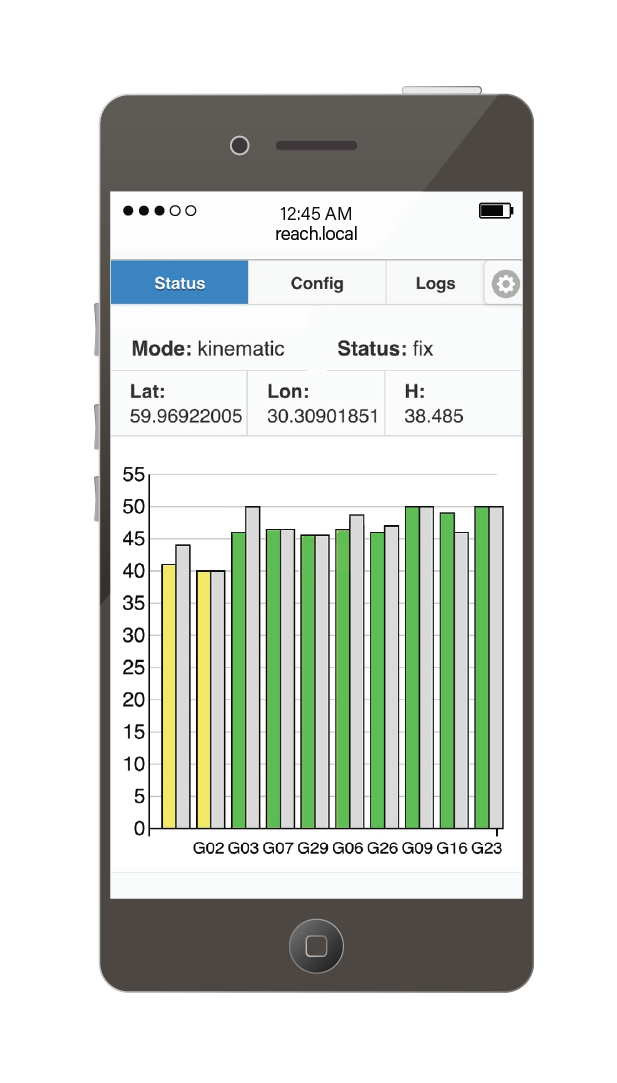
\includegraphics [scale=0.7] {SNR_chart}
  \caption{График уровней приема спутников}
  \label{img:latex}
\end{figure}

\subsection{Создание и чтение форм конфигурации. Модуль config.js} \label{subsect3_2_3}

Модуль \textbf{config.js} отвечает за работу с формами. Конфигурационные файлы RTKRCV, так же как и настройки STR2STR, которые задаются с помощью параметров запуска, имеют особенный синтаксис, особенно при задании входящих и исходящих потоков данных. Например, для того чтобы настроить RTKRCV на вывод координат через последовательный интерфейс, нужно выставить значения двух переменных

\begin{ListingEnv}[H]
  \caption{}
  \label{list:hwbeauty}
  \begin{lstlisting}
    outstr1-type       =serial
    outstr1-path       =ttyMFD2:57600:8:n:1:off
    outstr1-format     =llh
  \end{lstlisting}
\end{ListingEnv}

Задача модуля \textbf{config.js} отобразить эти самые настройки в удобном для чтения и изменения виде. При запуске с такими настройками RTKRCV обратится к \textbf{/dev/ttyMFD2} с настройкой скорости передачи данных 230400 бод. Пользователю неудобно работать с такой строкой и поэтому форма с настройками во вкладке \textbf{Config} превратит данную строку в раскрытую форму. Третья опция изменяет формат вывода на \textbf{llh}, или широта, долгота, высота и представлена отдельным селектором, следующей опцией. Результат отображения представлен на рисунке 3.2.

\begin{figure}[ht]
  \center
  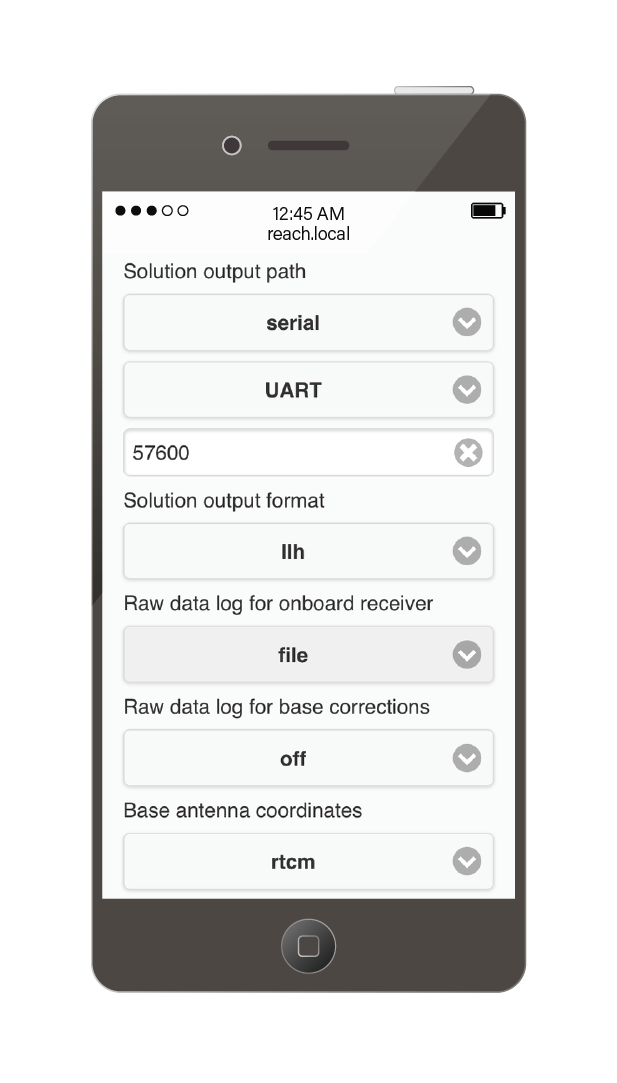
\includegraphics [scale=0.7] {Serial_form}
  \caption{Настройка вывода координат в формате llh в последовательный порт}
  \label{img:latex}
\end{figure}

Также, \textbf{config.js} выполняет обратную функцию - при изменении данных, нужно собрать данные формы в совместимые с RTKLIB строки. Для этого используются скрытые от пользователя строки, которые обновляются при любом изменении данных в форме.

\section{Сценарии взаимодействия фронтэнда и бэкенда} \label{sect3_3}
























